%% This is file `elsarticle-template-1a-num.tex',
%%
%% Copyright 2009 Elsevier Ltd
%%
%% This file is part of the 'Elsarticle Bundle'.
%% ---------------------------------------------
%%
%% It may be distributed under the conditions of the LaTeX Project Public
%% License, either version 1.2 of this license or (at your option) any
%% later version.  The latest version of this license is in
%%    http://www.latex-project.org/lppl.txt
%% and version 1.2 or later is part of all distributions of LaTeX
%% version 1999/12/01 or later.
%%
%% The list of all files belonging to the 'Elsarticle Bundle' is
%% given in the file `manifest.txt'.
%%
%% Template article for Elsevier's document class `elsarticle'
%% with numbered style bibliographic references
%%
%% $Id: elsarticle-template-1a-num.tex 151 2009-10-08 05:18:25Z rishi $
%% $URL: http://lenova.river-valley.com/svn/elsbst/trunk/elsarticle-template-1a-num.tex $
%%
%%\documentclass[preprint,12pt]{elsarticle}

%% Use the option review to obtain double line spacing
 \documentclass[preprint,review,12pt]{elsarticle}

%% Use the options 1p,twocolumn; 3p; 3p,twocolumn; 5p; or 5p,twocolumn
%% for a journal layout:
%% \documentclass[final,1p,times]{elsarticle}
%% \documentclass[final,1p,times,twocolumn]{elsarticle}
%% \documentclass[final,3p,times]{elsarticle}
%% \documentclass[final,3p,times,twocolumn]{elsarticle}
%% \documentclass[final,5p,times]{elsarticle}
%% \documentclass[final,5p,times,twocolumn]{elsarticle}

%% if you use PostScript figures in your article
%% use the graphics package for simple commands
%% \usepackage{graphics}
%% or use the graphicx package for more complicated commands
%% \usepackage{graphicx}
%% or use the epsfig package if you prefer to use the old commands
%% \usepackage{epsfig}

%% The amssymb package provides various useful mathematical symbols
\usepackage{amssymb}
%% The amsthm package provides extended theorem environments
%% \usepackage{amsthm}

%% The lineno packages adds line numbers. Start line numbering with
%% \begin{linenumbers}, end it with \end{linenumbers}. Or switch it on
%% for the whole article with \linenumbers after \end{frontmatter}.
%% \usepackage{lineno}

%% natbib.sty is loaded by default. However, natbib options can be
%% provided with \biboptions{...} command. Following options are
%% valid:

%%   round  -  round parentheses are used (default)
%%   square -  square brackets are used   [option]
%%   curly  -  curly braces are used      {option}
%%   angle  -  angle brackets are used    <option>
%%   semicolon  -  multiple citations separated by semi-colon
%%   colon  - same as semicolon, an earlier confusion
%%   comma  -  separated by comma
%%   numbers-  selects numerical citations
%%   super  -  numerical citations as superscripts
%%   sort   -  sorts multiple citations according to order in ref. list
%%   sort&compress   -  like sort, but also compresses numerical citations
%%   compress - compresses without sorting
%%
%% \biboptions{comma,round}

% \biboptions{}
\usepackage{textcomp, fixltx2e}


 \journal{Journal of Analytical and Applied Pyrolysis}

\begin{document}

\begin{frontmatter}

%% Title, authors and addresses

%% use the tnoteref command within \title for footnotes;
%% use the tnotetext command for the associated footnote;
%% use the fnref command within \author or \address for footnotes;
%% use the fntext command for the associated footnote;
%% use the corref command within \author for corresponding author footnotes;
%% use the cortext command for the associated footnote;
%% use the ead command for the email address,
%% and the form \ead[url] for the home page:
%%
%% \title{Title\tnoteref{label1}}
%% \tnotetext[label1]{}
%% \author{Name\corref{cor1}\fnref{label2}}
%% \ead{email address}
%% \ead[url]{home page}
%% \fntext[label2]{}
%% \cortext[cor1]{}
%% \address{Address\fnref{label3}}
%% \fntext[label3]{}

\title{Following beech litter decomposition with analytical pyrolysis: Inter-site variance, decomposition trends and stoichiometric controls}

%% use optional labels to link authors explicitly to addresses:
%% \author[label1,label2]{<author name>}
%% \address[label1]{<address>}
%% \address[label2]{<address>}

\author{}

\address{}

\begin{abstract}
%% Text of abstract

\end{abstract}

\begin{keyword}
%% keywords here, in the form: keyword \sep keyword

%% MSC codes here, in the form: \MSC code \sep code
%% or \MSC[2008] code \sep code (2000 is the default)

\end{keyword}

\end{frontmatter}
\pagestyle{empty}

%%
%% Start line numbering here if you want
%%
% \linenumbers

%% main text

\section{Introduction}


Analytical pyrolysis is frequently applied to characterize natural organic polymers like soil organic matter, dissolved organic matter or plant ligno-cellulose. Plant derived compounds make up an important part of pyrolysis products found. The relative abundances of such markers were shown to hold key information on past climates and decomposition conditions \cite{i.e. Kuder1998, Schellekens2009, Schellekens2011}. Interestingly, only a handful of Pyr-GC/MS studies tracing changing pyrolysis markers during decomposition processes  were published. 

%In several recent studies, fossil pyrolysis products is often based on their origin from plant polymers. \cite{Kuder1998} analyzes subfosil plant particles and \cite{Schellekens2009, Schellekens2011} soil organic matter (SOM) fractions to reconstruct past climate and vegetation from a peat profile.

[To our best knowledge] The only published work directly studying the decay of plant leaf litter is \cite{Franchini2002}. In a number of cases, litter was mixed with soils to follow decomposition by GC/MS. Straw was incubated with n.

the decomposition dynamics, from which pyrolysis products result are far from elucidated. While assignment to major compounds classes (like ligin or carbohydrate) based on pyrolysis reaction mechnisms is common, little is known on whether the composition of individual pyrolysis products within this groups yields information. 

The lack of reliable methods for lignin quantification led to the application of analytical pyrolysis as a cheap and fast method to estimate fibre content and nutrient quality of forage material. 

 n. ...

This study compares pyrograms of beech litter from different site after up to 15 month of decomposition. Beech litter has an exceptionally slow decomposition both in nature \citep{Klotzbucher2011} and in our climate chamber experiment. However, several  

Inter-site comparison of litter traits within a given species give a 

\section{Material and Methods}

We analyzed samples from a litter decomposition experiment with Pyr-GC/MS. Beech litter from 4 different sites in Austria was collected in October 2008, cut to pieces \textless 0.5 cm, homogenized, sterilized and inoculated with a common inoculate for all sites. Litter was incubated in a climate chamber at 15 \textdegree C and was kept at 60 \% moisture \citep{Wanek2010}.
Total mass loss after 15 month was between 7 and 15 \%.
Accumulated respiration after 6 month accounts for nn.to nn\% of the litter carbon pool, after 15 month between n and n\.

Pyrolysis-GC/MS was performed on a Pyroprobe 5250 pyrolysis system (CDS Analytical) coupled to a Thermo Trace gas chromatograph and a DSQ II MS detector (both Thermo Scientific) equipped with a carbowax colomn (Supelcowax 10, Sigma-Aldrich). 2-300 \textmu g dried and finely ball-milled litter were heated to 600\textdegree C for 10 seconds in helium atmosphere. The temperature of the valve oven and the transfer line to the GC injection port were set to 250\textdegree C,a 10x split injection was applied with the injector heated to 240\textdegree C. GC Oven temperature was constant at 50 \textdegree C for 2 minutes, followed by an increase of 7\textdegree C/min to a final temperature of 260 \textdegree C, which was held for 15 minutes. The transfer line was heated to 270 \textdegree C. The MS detector was set for electron ionization at 70 EV, the ion source was heated to 270\textdegree C. Detection was set to cycle between m/z 20 and 300 with a cycle time of 0.3 seconds.

Peaks were assignment was based on NiSt 05 MS library and comparison with reference material measured. 133 peaks were identified and selected for integration due to their hight abundance or diagnostic value. For each peak between one and four dominant mass fragments selected for high abundance and specificity were integrated (i.e. \cite{Schellekens2009, Kuder1998}). Peak areas are stated as \% of the sum of all integrated peaks of a sample. 

Pyrolysis products were assigned to their substances of origin by comparison to reference material, structural similarity and in accordance with literature (\cite{Ralph1991a, Schellekens2009, Chiavari1992}[more lit!]). The sum of all peak areas of the pyrolysis products of a class was calculated based on total ion current (TIC) peak areas. TIC peak areas are (1) less specific as areas of specific MS fragments and (2) integration was not possible for all peaks a/o all samples. Therefore a MS response factor Rf was calculated for each detected substance:

\begin{equation}
Rf = median (\frac{TIC peak area}{specific MS fragment peak area})
\end{equation}

Peak areas were multiplied by Rf before addition to calculate percentages of TIC area without loosing the specifity of integrating single m/z traces.

% However, during interpretation, we found little difference between direct sums of the integrated fragments and sums of corrected areas, indicating little sensitivity for exact 

Relative peak areas in both integrations are different from weight\%, but allow tracing of accumulation/depletion of these substance classes during decomposition \citep{Schellekens2009}. 


\subsection{Statistical analysis}
All statistical analyses were performed with the software and statistical computing environment R using the R package ``vegan'' \citep{Oksanen2011}. If not mentioned otherwise, results were considered significant, when p\textless 0.05. All correlations refer to Pearson correlations.
All data presented was tested for significant differences between harvests and litter types. Normal distribution assumed but could not be tested due to the small number of cases per treatment (n=4-5). A substantial part of variables had heterogeneous variances when tested ẃith Levene's test. Therefore, (one-way) Welch anova was used to calculate significant differences between harvests within each litter type and litter types within each harvest (alpha=0.05). For post-hoc group assignment, paired Welch's t-tests with Bonferroni corrected p limits were used. Principal component analysis was performed using vegan function ``rda'' scaling variables.
\section{Results}

\subsection{Pyrolysis products}

A total of 128 pyrolysis products were identified and quantified.

\subsection{Lignin and other Phenoles}

Pyrolysis products of lignin are 2-methoxyphenol (guaiacol) and 2,6-dimethoxyphenol (syringol) with alkyl chains of up to 3 C-atoms at C$_4$.

A total of 38 phenolic pyrolysis products were identified, 15 of which had guaiacol-, 13 syringol-, and 10 non-methoxylated ring systems. Guaiacol/Syringol (G/S) ratios were tightly (all R=0.68-0.94, p<0.001) correlated between the more abundant side chains (-H, -CH$_3$, -CH$_2$CH$_3$, -CH=CH$_2$, -CH$_3$CH=CH$_2$). This correlation is weaker or non-significant for less abundant side chains (-CHO, -CH$_2$CH$_2$CHO), probably due to higher variances in their detection [see fig.,]. 

Part of non-methoxylated phenols pyrolysis products (side chains -CH$_2$CH$_3$, -CH$_2$CH$_2$CH$_3$ -CH$_3$CH=CH$_2$)show clear structural similarity to pyrolysis products of lignin, suggesting that they are pyrolysis products of p-hydroxypropanylphenol based lignin. Other side chains (-H, -CH$_3$, -CHO) are less specific and are reported for other sources, although in small amounts. Furthermore, some of the phenolic compounds (i.e. hydroxyquinone) are not lignin derived. 

In both syringol and gaiacol the ratio between the abundances of pyrolysis products is the same.

Guaiacol to Syringol ratios were constant over decomposition time. 

Most important differences between sites were observed in the ratio between Guaiacol


The pattern of abundances of different side chains was the same for guaiacol and syringol derived compounds. Fig \ref{sidechainratios}shows that the ratios between 15 pairs of side chains are highly significant in guaiacol and syringol lignin based pyrolysis products. However, there are some site-specific differences in these patterns: the abundance of -H and -CH$_3$ side chains relative to other side chains is different between the litter types, but consistent between guaiacol and syringol derivatives. 
  de chains with oxygen based functional groups were present, but in abundances much lower than the before mentioned. 

\cite{Kuder1998, Schellekens2009} use the Guaiacol+Syringol to C$_3$-Gaiacol+Syringol ratio as an indicator for ?aerobic/anaerobic degradation. 

\subsection{N compounds}

11 N containing compounds were identified. They were tightly correlated to each other, especially methylindol and indole (R=0.98, p\textless 0.05?0.001?). and 6 pyridin and pyrrol derivatives (all R \textgreater 0.9, p\textless 0.05?0.001?). The two groups were correlated to each other (R = 0.77-0.87, p\textless 0.05?0.001?). 2 pyrrol derivatices (N-methyl-pyrrol and methylpyrrol[II]) and pyridol showed were not or less strict correlated to the other compounds, due to low abundance. Furthermore, all N markers except the three mentioned before were correlated to litter N content (R \textgreater 0.81, p \textless 0.001.


While N compounds generally increase in 

Pyridol looses during first three month, then follows generall N trend.

\subsection{Carbohydrates}
In total, 42 carbohydrate derived pyrolysis products were identified either by their structure or by comparison to reference material (celluluse, xylran, glucose, ...). Unlike lignin or N compounds, carbohydrate pyrolysis products do not follow a common trend, but - reflecting the differences within this group, 


Furanmethanol shows an especially high degradation rate, loosing 15 to 30 \% of it's initial contribution to the total peak area over 15 month.


\section{Discussion}

\subsection{Lignin side chains}
Until now, studies following lignin degradation with Pyr-GC/MS \citep{ were focusing on changes between the frequency of lignin pyrolysis products, only the ratio between guaiacol/syringol/phenol based ring system was investigated. We found substantial differences in the frequency of different lignin side chains between litter collected at different sites. We found that these differences remained nearly constant during during 15 month of litter decomposition. 

\section{Conclusions}


\section{Acknowledgements}

%% The Appendices part is started with the command \appendix;
%% appendix sections are then done as normal sections
%% \appendix

%% \section{}
%% \label{}

%% References
%%
%% Following citation commands can be used in the body text:
%% Usage of \cite is as follows:
%%   \cite{key}          ==>>  [#]
%%   \cite[chap. 2]{key} ==>>  [#, chap. 2]
%%   \citet{key}         ==>>  Author [#]

%% References with bibTeX database:

\bibliographystyle{elsarticle-num}
\bibliography{library}

%% Authors are advised to submit their bibtex database files. They are
%% requested to list a bibtex style file in the manuscript if they do
%% not want to use model1a-num-names.bst.

%% References without bibTeX database:

% \begin{thebibliography}{00}

%% \bibitem must have the following form:
%%   \bibitem{key}...
%%

% \bibitem{}

% \end{thebibliography}
\newpage

\section{Figures}
\begin{figure}
  \caption{A comparison of the ratios between 15 pairs of side chains in guaiacol and syringol derived pyrolysis products.}
  \centering
    \includegraphics[width=12cm]{sidechainratios_new.pdf}
  \label{sidechainratios}
\end{figure}





\begin{figure}[p!]
  \caption{G/Sy ratio for 5 pairs of compounds with different side chains.}
  \centering
    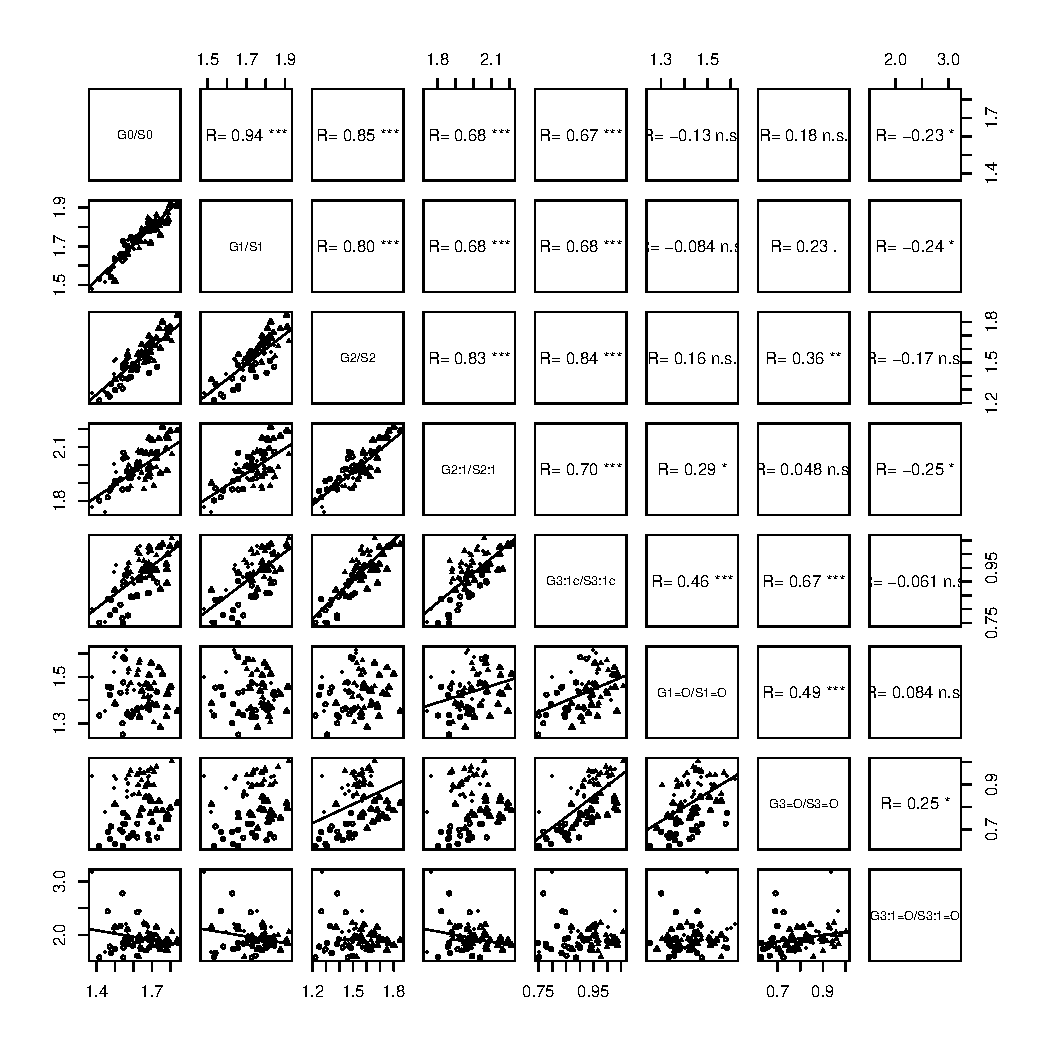
\includegraphics[width=0.5\textwidth]{G_Sy_ratio.pdf}
\end{figure}

\section{Tables}

\begin{table*}[p!]
\begin{center}
{\tiny
\begin{tabular}{llclcccccc}
code & name & ring & side chain & RT & MW & m/z & class & origin&Rf\\
\hline
Ph0&		Phenol&				Phenol&		-H&			21.02&		&	&		ph&	Ph& 	1.717828\\
Ph1a&		4-Methylphenol&			Phenol&		-CH$_3$&		22.11&		&	&		ph&     Ph&	1.700271\\
Ph1b&		3-Methylphenol&			Phenol&		-CH$_3$&		22.22&		&	&		ph&	Ph&	1.353149\\
Ph2&		Ehtylphenol&			Phenol&		-CH$_2$CH$_3$&		23.38&		&	&		ph&	Ph&	1.356640\\
Ph3:1a&		Propenylphenol&			Phenol&		-CH$_2$CH=CH$_2$&	26.93&		&	&		ph&	Ph&	5.133600\\
Ph3:1b&		Propenylphenol&			Phenol&		-CH$_2$CH=CH$_2$&	27.76&		134&	133+134&	ph&	Ph&	4.779586\\
Ph3&		Propylphenol&			Phenol&		-CH$_2$CH$_2$CH$_3$&	31.11&		&	&		ph&	Ph&	1.387483\\
Ph4&		?Butylphenol&			Phenol&		-C$_4$H$_9$&		31.86&		&	&		ph&	Ph&	2.417611\\
ph1=O&		4-Hydroxybenzaldehyde&		Phenol&		-CHO&			32.70&		122&	121+122&	ph&	Ph&	b.d.\\
Ph-OH&		Hydroquinone&			Phenol&		-OH&			33.40&		&	&		ph&	Ph&	2.143460\\
\\
G0&		Guaiacol&			Guaiacol&	-H&			18.87&		124&	109+124&	g&	L&	2.48\\
G1&		Methylguaiacol&			Guaiacol&	-CH$_3$&		20.32&		138&	123+138&	g&	L&	1.93\\
G2&		Ethylguaiacol&			Guaiacol&	-CH$_2$CH$_3$&		21.4&		152&	137+152&	g&	L&	2.18\\
G3:1a&		Propenylguaiacol[1]&		Guaiacol&	-CH$_2$CH=CH$_2$&	23.29&		164&	149+164&	g&	L&	3.30\\
G2:1&		Ethylenguaiacol&		Guaiacol&	-CH=CH$_2$&		23.69&		150&	135+150&	g&	L&	2.05\\
G3:1b&		Propenylguaiacol[2]&		Guaiacol&	-CH$_2$CH=CH$_2$&	24.48&		164&	149+164&	g&	L&	14.20\\
G3:1c&		Propenylguaiacol[3]&		Guaiacol&	-CH$_2$CH=CH$_2$&	25.66&		164&	149+164&	g&	L&	5.01\\
G1=O&		Gaiacolaldehyde&		Guaiacol&	-CHO&			28.4&		152&	109+152&	g&	L&	b.d.\\
G3&		Propanylguaiacol&		Guaiacol&	-CH$_2$CH$_2$CH$_3$&	28.72&		166&	137+166&	g&	L&	1.47\\
G3=0-OH&	Oxo-hydroxy-propanylguaiacol&	Guaiacol&	-CH(OH)-CH$_2$-CHO&	28.77&		182&	182&		g&	L&	20.45\\
G2=O&		Oxo-ethylguaiacol&		Guaiacol&	-CH$_2$CHO&		29.2&		166&	151+166&	g&	L&	1.69\\
G3=O&		Oxo-propanylguaiacol&		Guaiacol&	-CH$_2$CH$_2$CHO&	29.36&		180&	137+180&	g&	L&	1.70\\
GAc&		Guaiacylacetic acid&		Guaiacol&	-CH$_2$COOH&		32.88&		182&	137+182&	g&	L&	2.04\\
G3:1=O&		Oxo-propenylguaiacol&		Guaiacol&	-CH=CH-CHO&		35.3&		178&	135+178&	g&	L&	4.12\\
G3:1-OH&	Hydroxy-propenylguaiacol&	Guaiacol&	-CH=CH-CH$_2$OH&	37.1&		180&	137+180&	g&	L&	2.08\\
\\
S0&		Syringol&			Syringol&	-H&			24.58&		154&	139+154&	sy&	L&	2.37\\
S1&		Methylsyringol&			Syringol&	-CH$_3$&		25.67&		168&	153+168&	sy&	L&	b.d.\\
S2&		Ethylsyringol&			Syringol&	-CH$_2$CH$_3$&		26.39&		182&	167+182&	sy&	L&	1.70\\
S3:1a&		Propenylsyringol[1]&		Syringol&	-CH$_2$CH=CH$_2$&	27.97&		194&	179+194&	sy&	L&	4.58\\
S2:1&		Ethylensyringol&		Syringol&	-CH=CH$_2$&		28.37&		180&	165+180&	sy&	L&	5.10\\
S3:1b&		Propenylsyringol[2]&		Syringol&	-CH$_2$CH=CH$_2$&	28.91&		194&	179+194&	sy&	L&	2.71\\
S3:1c&		Propenylsyringol[3]&		Syringol&	-CH$_2$CH=CH$_2$&	30.16&		194&	194+179&	sy&	L&	3.76\\
S1=O&		Syringolaldehyd&		Syringol&	-CHO&			32.68&		182&	139+182&	sy&	L&	7.20\\
S3&		Propanylsyringol&		Syringol&	-CH$_2$CH$_2$CH$_3$&	33.15&		196&	181+196&	sy&	L&	3.05\\
S3=O-OH&	Oxo-hydroxy-propanylsyringol&	Syringol&	-CH(OH)-CH$_2$-CHO&	32.8&		212&	212&		sy&	L&	b.d.\\
S3=O&		Oxo-propanylsyringol&		Syringol&	-CH$_2$CH$_2$CHO&	33.32&		210&	167+210&	sy&	L&	1.64\\
SAc&		Syringylacetic acid&		Syringol&	-CH$_2$COOH&		38.78&		212&	212&		sy&	L&	4.78\\
S3:1=O&		Oxo-propenylsyringol&		Syringol&	-CH=CH-CHO&		43.06&		208&	165+208&	sy&	L&	2.96\\
\hline
\end{tabular}}
\caption{Lignin and phenol pyrolysis products.}
\end{center}
\label{tab:ligprod}
\end{table*}

\begin{table*}[p!]
\begin{center}
{\tiny
\begin{tabular}{llclcccccc}
code & name & ring & side chain & RT & MW & m/z & class & origin&Rf\\
F0&		Furan&				Furan&			&		2.35&		68&	39+68&		f&	C&	1.19\\
F1a&		Methylfuran&			Furan&			&		2.74&		82&	81+82&		f&	C&	1.00\\
F1b&		Methylfuran&			Furan&			&		2.91&		82&	81+82&		f&	C&	b.d.\\
F1.1a&		Dimethylfuran&			Furan&			&		3.43&		96&	95+96&		f&	C&	b.d.\\
F1.1b&		Dimethylfuran&			Furan&			&		3.66&		96&	95+96&		f&	C&	1.10\\
F2:1&		Vinylfuran&			Furan&			&		5.01&		94&	65+94&		f&	C&	2.59\\
F1=Oa&		3-Furaldehyd&			Furan&			&		11.57&		96&	95+96&		f&	C&	1.65\\
&		2(5H)Furanon&			Furan&			&		11.69&		98&	55+98&		f&	C&	2.41\\
F1=Ob&		2-Furaldehyd&			Furan&			&		12.22&		96&	95+96&		f&	C&	1.67\\
FAc&		Acetylfuran&			Furan&			&		12.99&		110&	95+110&		cp&	C&	2.38\\
% "11","f11","5-Methyl-2-furancarboxaldehyde",14.23,"110","109+110","f","C",2.440815327,FALSE,NA,NA
% "12","cp12","Butyrolactone",15.22,"86","56+86","cp","C",12.373827545,FALSE,NA,NA
% "13","cp13","Furanmethanol",15.61,"98","98","cp","C",5.206772312,FALSE,NA,NA
% "14","f14","5-Methyl-2(5H)-furanone",16.06,"98","55+98","f","C",3.9163635165,FALSE,NA,NA
% "15","f15","5-hydroxymethylfuran1--carboxaldehyde",27.51,"126","97+126","f","C",2.171627102,FALSE,NA,NA
% "30","cp1","2-Oxopropanoic Acid, ME",7.92,"102","43+102","cp","C",0.579144112,FALSE,NA,NA
% "31","cp2","1-Hydroxypropanone",9.24,"74","43","cp","C",1.428699657,FALSE,NA,NA
% "32","cp3","Propanoic acid, ME",12.1,"102","43+102","cp","C",1.442887015,FALSE,NA,NA
% "33","f41","unknown carbohydrate 1",19.06,"","58+86+114","f","C",1.830393883,FALSE,NA,NA
% "34","cp5","unknown carbohydrate 2",19.35,"","98+126","cp","C",5.34990526,FALSE,NA,NA
% "35","f61","unknown carbohydrate 3",21.77,"","116","f","C",0,FALSE,NA,NA
% "36","cp7","unknown carbohydrate 4",22.33,"","44","cp","C",3.336083454,FALSE,NA,NA
% "37","f81","unknown carbohydrate 5",26.18,"","57+69","f","C",1.153004104,FALSE,NA,NA
% "38","f91","unknown carbohydrate 6",31.67,"","73+135","f","C",7.590107005,FALSE,NA,NA
% "39","f10","laevoglucosan",40.44,"","60+73","f","C",0,FALSE,NA,NA
\\

% "40","cp11","10.26_2-cyclopenten-1-one",10.26,"82","53+54+52","cp","C",2.020538261,FALSE,NA,NA
% "41","cp21","10.51_2-methyl-2-cyclopenten-1-one",10.51,"96","53+96","cp","C",2.36623591,FALSE,NA,NA
% "42","cp31","13.31_3-methyl-cyclopentanone",13.31,"","67+96","cp","C",4.0617533325,FALSE,NA,NA
% "43","cp4","13.69_dimethylcyclopentenone",13.69,"110","67+95+110","cp","C",1.6276422925,FALSE,NA,NA
% "44","cp51","14.44_2-cyclopenten-1,4-dione",14.44,"96","54+68+96","cp","C",1.6790668675,FALSE,NA,NA
% "45","cp6","17.51_1,2-cylopentandione",17.51,"98","55+98","cp","C",2.2214713485,FALSE,NA,NA
% "46","cp71","18.14_2-cyclopenten-1-one,_-2-hydroxy-3-me",18.14,"98","98","cp","C",15.95856595,FALSE,NA,NA
% "47","cp8","18.42_1,2-cyclopentanedione,_-3-methyl-",18.42,"112","69+112","cp","C",2.735582125,FALSE,NA,NA
% "66","f31","unknown_furan_6.36",NA,"","","f","C",1.9282758805,FALSE,NA,NA
% "67","cp41","cyclopentanone_6.99",NA,"","","cp","C",0,FALSE,NA,NA
% "71","f82","methylfurane2_7.64",NA,"","","f","C",2.0044374263,FALSE,NA,NA
% "76","cp131","1-Hydroxy-2-propanone_ch_10.69",NA,"","","cp","C",2.4592896545,FALSE,NA,NA
% "77","cp14","unknown_ch_11.38",NA,"","","cp","C",4.6641589255,FALSE,NA,NA
% "80","cp17","unknown_ch_15.56",NA,"","","cp","C",119.6856377927,FALSE,NA,NA
% "82","cp19","unknown_ch_16.17",NA,"","","cp","C",2.5775022825,FALSE,NA,NA
% "83","cp20","unknown_17.67",NA,"","","cp","C",1.1554018384,FALSE,NA,NA
% "123","cp15","Acetaldehyde",2.06,"44","29+44","cp","C",1.044112118,FALSE,NA,NA
\hline
\end{tabular}}
\caption{Carbohydrate pyrolysis products.}
\end{center}
\label{tab:chprod}
\end{table*}

\end{document}

%%
%% End of file `elsarticle-template-1a-num.tex'.
